\documentclass{article}
\usepackage{amsmath}
\usepackage{amssymb}
\usepackage{graphicx}
\usepackage{hyperref}
\usepackage{enumitem}
\usepackage{times}
\usepackage{breqn}
\usepackage{float}
\usepackage{fancyhdr,graphicx,amsmath,amssymb}
\usepackage[ruled,vlined]{algorithm2e}
\include{pythonlisting}

\title{Algorithms Homework 9}
\author{Koi Stephanos}
\date{November 2019}

\begin{document}

\maketitle

\begin{enumerate}
\item
    To prove that the subgraph problem is NP, we must show that, given a certificate, we can verify a solution. In this case, if we are given a labeled subgraph (both edges and nodes) as a certificate, we can check to see if those nodes and edges are indeed in the graph.
    
    To prove that it is NP-c, we must additionally show that we can use the subgraph problem to solve a different NP-c problem. Here, we will use the largest clique problem. This is solvable via the subgraph, because we can pass in a subgraph that is a clique, and if it is contained, we know there must be a clique of that size. By testing different sizes of cliques, we will eventually find a match and that gives us the largest clique in the graph.

\item
    The 0-1 integer-programming problem has an \(m\) x \(n\) integer matrix \(A\), and an integer \(m\)-vector \(b\) and asks whether there is an \(n\)-vector in \(A\) that is \(\leq b\). This is clearly NP, because given \(b\), if we receive a \(n\)-vector of \(A\) as a certificate, we can compare that to \(b\) to confirm.
    
    To prove this is NP-c, we need to represent this problem as a different NP-c problem, and here we can use the 3-CNF-SAT. In 3-CNF-SAT, we have a series of Or gates with 3 inputs all running into an And gate. Our circuitry is satisfied if the And outputs a 1, which means at least one of the inputs for each Or gate must be a 1. This itself can be represented as an integer program, which means that a solution to the 0-1 integer programming problem can indirectly be used to solve the 3-CNF-SAT problem.
    
\item
    The set-partition problem asks if given a set of number \(S\), can you find two subsets whose total sum is equal. This is clearly NP, because given a subset as a certificate, you can just take that sum and see if it equals half of the sum of \(S\).
    
    To show it is NP-c, we can use the subset problem, which is similar in that given a set of numbers \(S\) and a number \(W\), can you find a subset of \(S\) that equals W. If we just make our \(W\) equal to half the sum of \(S\), we have reduced that problem to the set-partition problem, which means it must be Np-c.
    
\item
    The Hamiltonian-path problem is clearly NP, because given a graph and a Hamiltonian-path as a certificate, we can verify whether or not that path exists in the graph.
    
    We can use the Hamiltonian-cycle problem to show this is NP-c. The Hamiltonian-path is just a Hamiltonian-cycle without a connection between the two ends of the path. On any given graph that has a Hamiltonian-path, you can check for a cycle by seeing if the two ends of the path share an edge, if so, you have your cycle. So if we have a method that gives us all the Hamiltonian-paths for a graph, we can test through those paths for a cycle to solve the Hamiltonian-cycle problem.

\item  
    SKIP
    
\item
    \hspace*{.5em}\begin{minipage}{.99\linewidth}
        \begin{algorithm}[H]
            \SetAlgoLined
            \KwIn{Graph}
            \KwResult{Colors Graph vertices with 2 colors if possible, false if not}
            \BlankLine
            startNode = Graph.randomNode()\;
            startNode.color = A\;
            nextNode\;
            \BlankLine
                \While{Graph.hasUncoloredNode() == true}{
                    nextNode = Graph.findUncoloredNodeWithColoredNeighbor()\;
                    \If{nextNode is null} {
                        return false\;
                    }
                    \ElseIf{nextNode.coloredNeighbor.color == A} {
                        nextNode.color = B\;
                    }
                    \Else{
                        nextNode.color = A\;
                    }
                }
            \caption{Graph 2-Coloring}
        \end{algorithm}
    \end{minipage}
    
\item
    \(\pi = \{0,0,1,2,0,1,2,0,1,2,0,1,2,3,4,5,6,7,8\}\)
    
\item
    To Do
    
\item
    \hspace*{.5em}\begin{minipage}{.99\linewidth}
        \begin{algorithm}[H]
            \SetAlgoLined
            \KwIn{Jobs, Machines}
            \KwResult{All jobs scheduled}
            \BlankLine
                \While{Jobs.notEmpty() == true}{
                    \ForEach {m in Machines} {
                        \If{m.isIdle() == true}{
                            m.assignJob(Jobs.pop())\;
                        }
                    }
                }
            \caption{Greedy Parallel Machine Scheduling}
        \end{algorithm}
    \end{minipage}
    
    Where \(m\) is number of jobs and \(n\) is number of processors, our running time for this algorithm is \(O(n*m)\).
\item
    A min-heap and a binary search tree are similar in that they organize data. A min-heap uses the smallest value as the root, and every child must be smaller than its parent. A binary search tree is similar, but split left and right, such that all elements in the left subtree are smaller than the root and all elements in the right subtree are larger. 
    
    This distinction, however, means that a min-heap can not print in sorted order in \(O(n)\) time, because there is no guarantee that values on the left side of the heap are less than the right side of the heap or vice versa. As a result, merely traversing the structure alone will not result in sorted data.
    
\item
\hspace*{.5em}\begin{minipage}{.99\linewidth}
    \begin{figure}[H]
        \centering
        \textbf{Red-Black Tree}\par\medskip
        \centerline{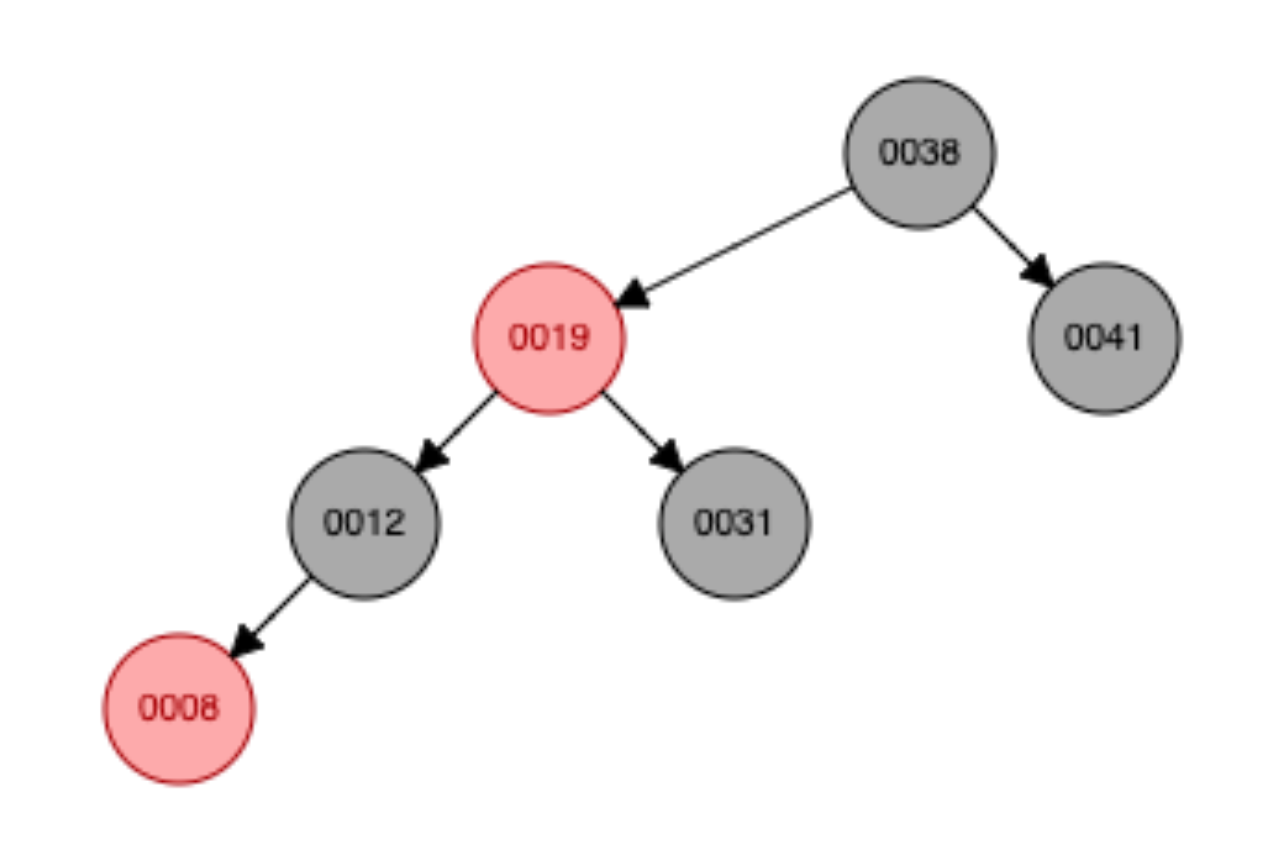
\includegraphics[width=10cm]{redBlackTree.png}}
    \end{figure} 
    \end{minipage}

\end{enumerate}
\end{document}